% Template for ICME 2019 paper; to be used with:
%          spconf.sty  - ICASSP/ICIP/ICME LaTeX style file, and
%          IEEEbib.bst - IEEE bibliography style file.
% --------------------------------------------------------------------------
\documentclass{article}
\usepackage{spconf,amsmath,epsfig}

\pagestyle{empty}


\begin{document}\sloppy
\topmargin=0mm

% Example definitions.
% --------------------
\def\x{{\mathbf x}}
\def\L{{\cal L}}


% Title.
% ------
\title{BUILDING EFFECTIVE SHORT VIDEO RECOMMENDATION}
%
% Single address.
% ---------------
\name{Yang Liu$^1$, Cheng Lyu$^1$, Zhiyuan Liu$^1$, and Dacheng Tao$^2$}
\address{$^1$School of Transportation, Southeast University\\
$^2$UBTECH Sydney Artificial Intelligence Centre and the School of
Information Technologies,\\the Faculty of Engineering and Information
Technologies, the University of Sydney\\
$^1$\{seu\_yangliu, cheng.lyu, zhiyuanl\}@seu.edu.cn,  $^2$dacheng.tao@sydney.edu.au}


\maketitle


%
\begin{abstract}
  How to build an effective personalized recommendation system is a challenging but highly valuable problem in social media services.
  This paper focuses on constructing a universal framework for short video recommendation by predicting the probability of finishing watching the entire video and pressing the `like' button. Four novel techniques are proposed to improve the prediction accuracy.
  Firstly, we present an Incremental Multi-Window Scanning approach to extract the features pertaining to the users' behaviors.
  Also, a User Interaction Behavior Hierarchy is designed to capture a larger quantity of information and reduce the computing time.
  Additionally, the model transfer is capable of transferring the knowledge learned by the model on other datasets to the final model.
  Lastly, a rank-based ensemble approach which is suitable for tasks based on the evaluation metric of AUC is proposed.
  Our method long ranked first in the final stage of ICME Short Video Understanding Challenge (Track1) before the revision of competition rule.
\end{abstract}
%
\begin{keywords}
Short video recommendation, model transfer, ensemble approach.
\end{keywords}
%

%%%%%%%%%%%%%%%%%%%%%%%%%%%%%%%%%%%%%%%%%%%%%%%%%%%%%%%%%%%%%
%%%%%%%%%%%%%%%%%%%%%%%%%%%%%%%%%%%%%%%%%%%%%%%%%%%%%%%%%%%%%


\section{Introduction}
\label{sec:intro}

With the increasing popularity of short-video-based social media platforms, personalized recommendation for videos have become an urgent yet challenging need. Instead of manually searching for the contents, it allows users to receive direct pushes of videos relating to their preferences. This is helpful in increasing user loyalty and facilitate the distribution of newly uploaded contents on the platform.
However, as summarized in \cite{sarwar_item-based_2001}, the two main obstacles in developing a recommendation algorithm are the scalability and quality. First, many traditional recommendation algorithms like k-nearest neighbors cannot handle large-scale dataset which is prevalent in the application scenarios nowadays. Second, a recommendation system with low recommending accuracy will reduce the users' satisfaction to the application.

\begin{figure}[h]
  \centering
  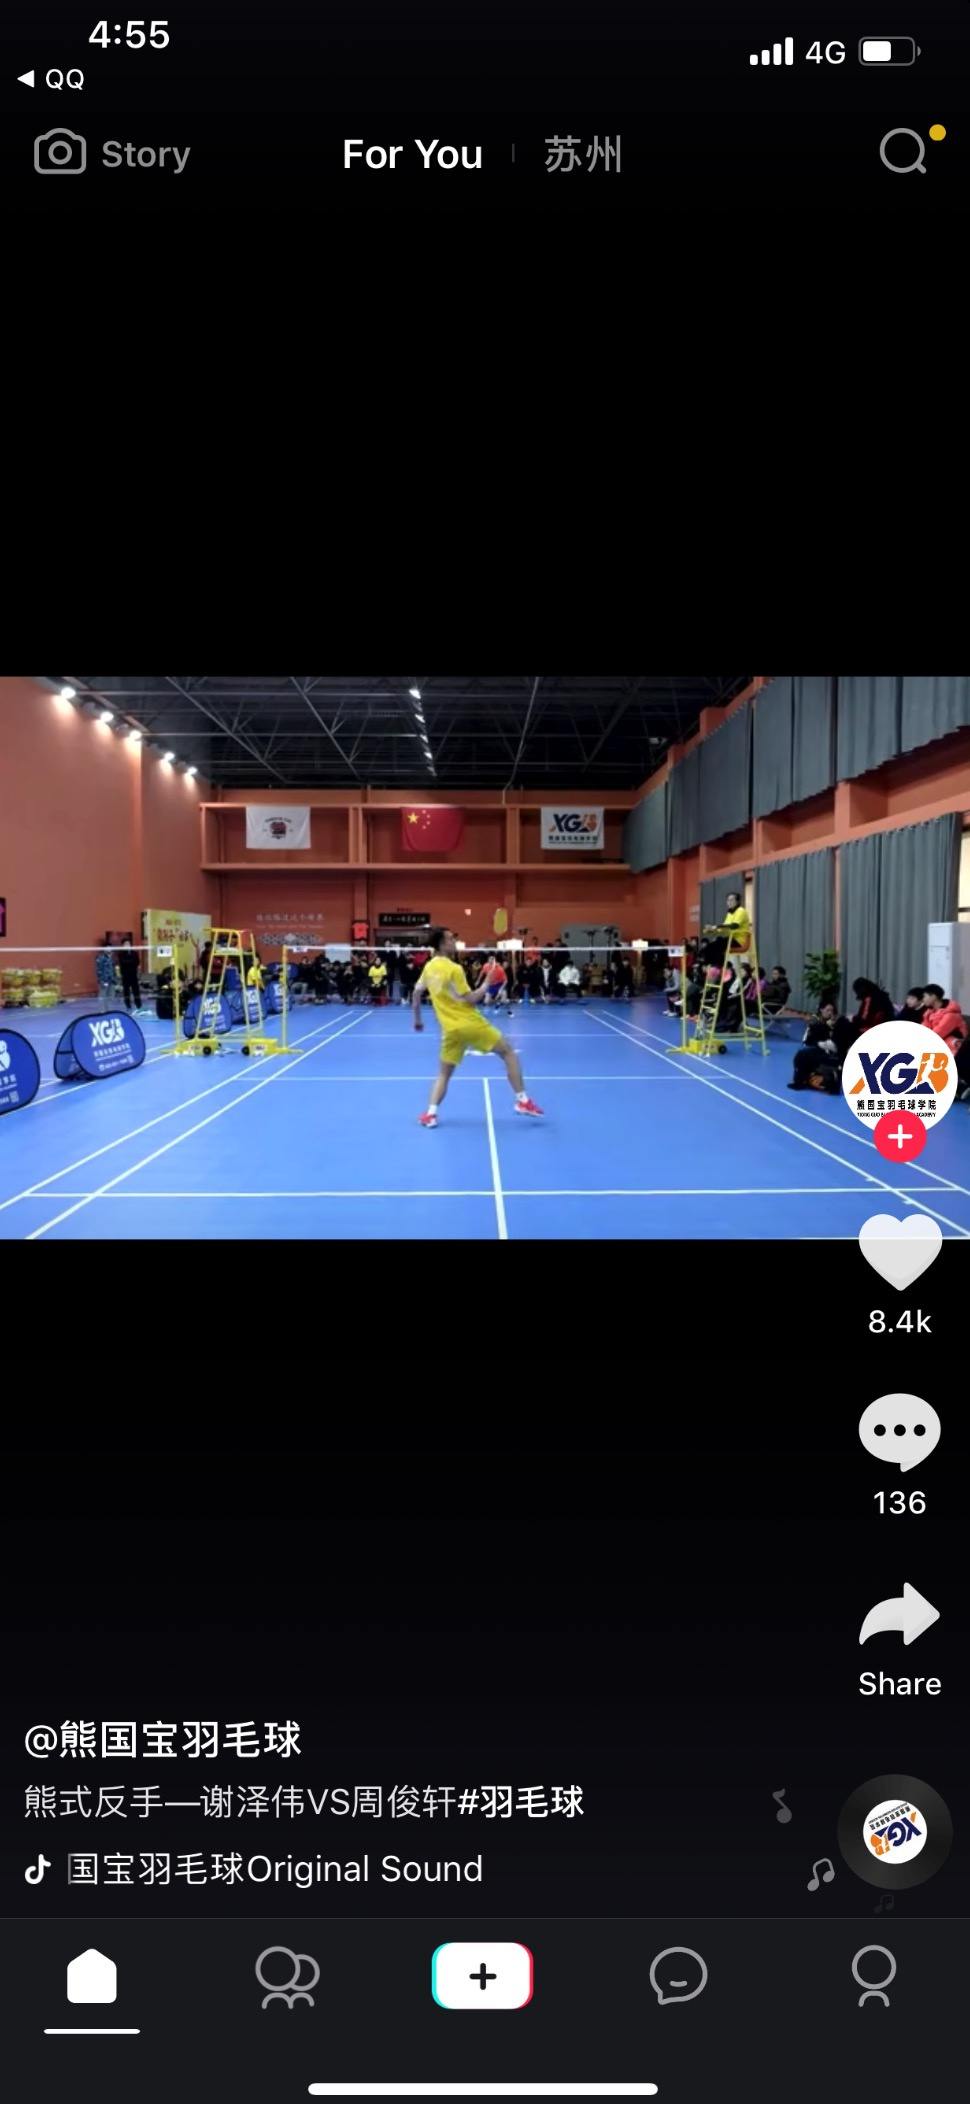
\includegraphics[width=4.2cm]{media/tiktok}
  \caption{A screenshot of the recommendation page on TikTok.}
  \label{fig:tiktok}
\end{figure}

TikTok, also named as Douyin, is one of the leading platforms in the market of short-video-based social media, where the millions of contents are being created, uploaded and shared every hour. To keep users entertained and attracted by the videos anytime when they launch the TikTok, the recommending strategy has to be based on the interests of users, which involves the users' behaviors and the understanding of video contents, including the subject, the editing quality, the background music, and the author.

Two representative strategies for personalized recommendation extensively studied in the past three decades are collaborative filtering (CF) and content-based filtering (CBF). Based on a user's preferences on items, CF matches him/her with the items liked by users, who share similar preferences \cite{sarwar_item-based_2001}. Singular vector decomposition (SVD) is popular for it is able to reduce the dimension while discover the similarities between items. In the famous Netflix prize challenge, \cite{koren_factorization_2008} won the game by merging the SVD-based latent factor model and the neighborhood model. A user-video graph was constructed in \cite{baluja_video_2008}, from which the co-view information can be deduced. Through an adsorption algorithm, the recommendation can be made on the basis of the propagation of neighboring preferences information. Attributes of the video contents, nevertheless, are often ignored in the CF-based recommendation frameworks.

Instead of focusing on users, the emphasis of CBF is placed on the characteristics of the items themselves. An online video recommendation framework was proposed in \cite{yang_online_2007,mei_videoreach:_2007}, where the relevance of multiple modalities of the video document was obtained, including textual, visual and aural information. Using an attention-based function, the relevance of different modalities was fused. In \cite{deldjoo_toward_2015}, the low-level visual features, which were directly extracted from the videos, were included in their model, for better understanding of the contents. 

To better capture the sophisticated relationships between users and videos, companies like Google are attempting to introduce deep learning into their recommendation system. For example, a two-stage recommendation framework, consisting of a candidate generation module and a deep ranking module in which both videos features and historic click-throughs were considered, was proposed by \cite{covington_deep_2016}.

In this paper, we addressed the short video recommendation problem and proposed an efficient universal framework. Four novel techniques, namely Incremental Multi-Window Scanning, User Interaction Behavior Hierarchy, Model Transfer and Rank-based Ensemble Method, are proposed to improve the prediction accuracy. The rest of paper is organized as follows. In the following section, the problem definition is first given. Then, we present the overview of the framework by elaborating the four proposed techniques. In Section 4, the experiment settings and the evaluation results are presented.

%%%%%%%%%%%%%%%%%%%%%%%%%%%%%%%%%%%%%%%%%%%%%%%%%%%%%%%%%%%%%
%%%%%%%%%%%%%%%%%%%%%%%%%%%%%%%%%%%%%%%%%%%%%%%%%%%%%%%%%%%%%

\section{Problem Definition}
\label{sec:problem-definition}

The overall objective of this research is to predict whether a user will finish watching specific video and whether they will click the `like' button for it.

The notations and problem are defined as follows:

Notation: User interaction behavior data $I$. A user interaction behavior record can be classified as user-related features, video-related features, and behavior-related data. User-related features contain the ID, city, and device of users. Video-related features contain the id, author, city, channel, background music, and duration of the video. For the behavior-related data, whether the users finished watching and liked the video, and the time they started watching are included.

Notation: Text feature $T$. The numerals and symbols were first removed from the video titles. Then, the titles were segmented into separate words. Finally, the frequency of each word was counted.

Notation: Visual feature $V$. This type of feature was extracted by the neural network, which transformed each video into a 128-dimensional vector.

Notation: Audio feature $A$. This feature set was also extracted by the neural network and was transformed into 128-dimensional vectors.

Problem: Given user id $u$ and video id $v$, build a machine learning model based on user interaction behavior data $I$, text feature $T$, visual feature $V$ and audio feature $A$, to predict whether a user will finish watching and like a specific short video.
%
\begin{equation}
  P_{i,\text{finish}} = P\big( \langle u_i, v_i \rangle | I,T,V,A \big)
\end{equation}
%
\begin{equation}
  P_{i,\text{like}} = P\big( \langle u_i, v_i \rangle | I,T,V,A \big)
\end{equation}
%
where $\langle u_i, v_i \rangle$ denotes the $i$-th user-video pair for
prediction, $P_{i,\text{finish}}$ is the probability of this user
finish watching the short video, and $P_{i,\text{like}}$ is the
probability of clicking the `like' button.


%%%%%%%%%%%%%%%%%%%%%%%%%%%%%%%%%%%%%%%%%%%%%%%%%%%%%%%%%%%%%
%%%%%%%%%%%%%%%%%%%%%%%%%%%%%%%%%%%%%%%%%%%%%%%%%%%%%%%%%%%%%

\section{Framework Overview}
\label{sec:framework-overview}

In this section, we present an overview of the proposed framework on short video recommendation system. This framework consists of four core components, namely Incremental Multi-Window Scanning, User Interaction Behavior Hierarchy, Model Transfer and Rank-based Ensemble Method.

\subsection{Incremental Multi-Window Scanning}
\label{sec:incremental-multi-window-scanning}

To predict the users’ behaviors on day $i-1$, the samples are usually constructed in the following way. We use the user interaction data of $m$ days, of which the data from the first $m-1$ days are used for feature extraction while the data from the last day was used for label extraction. Here, the range of days (i.e., $m$ days) used in feature extraction is called the time window size (i.e., $m$).

In the case of sufficient historical data, a time window that is too small (for example, one day) might result in too few user behaviors extracted. Moreover, it is highly possible that the selected day is distinct from other days in terms of user behavior due to festivals or important events. A larger time window size can have a larger receptive field, and, according, contribute to stronger robustness.

In this context, determining an appropriate window size is a key problem. This paper proposes an incremental multi-window scanning algorithm, which uses multiple time windows of different sizes to extract features pertaining to users’ behaviors instead of depending on a single window. The structure of the incremental multi-window scanning algorithm is illustrated in Fig.~\ref{fig:incre-multi-window-scan}.

\begin{figure}
  \centering
  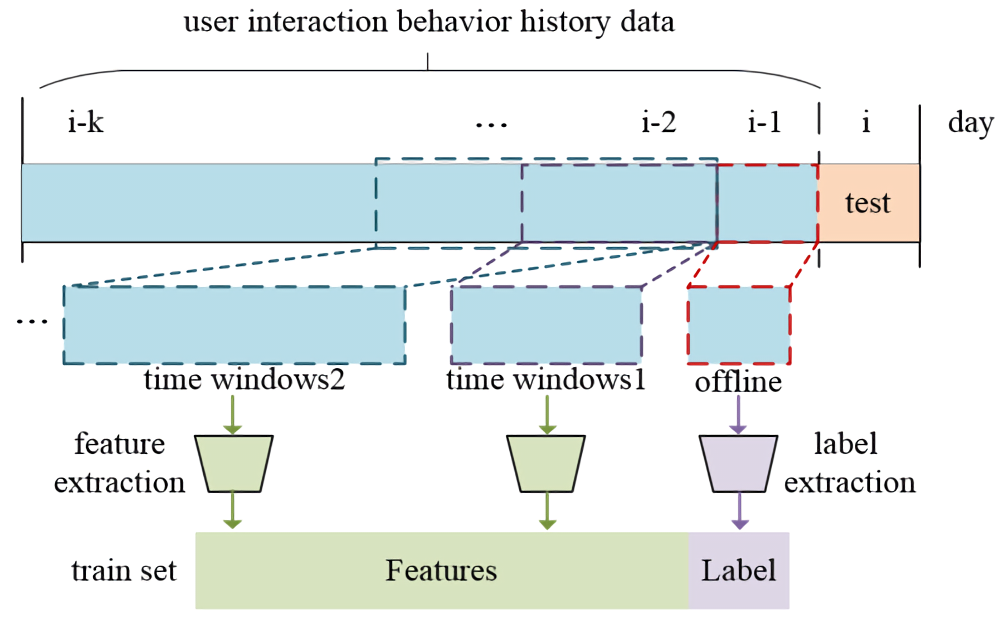
\includegraphics[width=8.5cm]{media/incre-multi-window-scan}
  \caption{Incremental multi-window scanning.}
  \label{fig:incre-multi-window-scan}
\end{figure}

% \setlength{\parskip}{0pt}
\subsection{User Interaction Behavior Hierarchy}
\label{sec:user-interaction-behavior-hierarchy}

Though, as mentioned in the previous section, a larger time window size leads to better performance, the computational cost, as well as the memory consumption, can also be substantial. We should note that out of the 30-40 million records of user behavior on each day, only 400 thousand of them relates to the ‘like’ behavior.

Inspired by the memory hierarchy in computer architecture, we designed a User Interaction Behavior Hierarchy (UIBH).
As shown in Fig.~\ref{fig:user-inter-behav-hierachy}, UIBH can be classified as complete user interaction behavior and core user interaction behavior, the former of which contains a wealth of information.
If, however, the historical data of one week or longer is used, the calculation time and memory consumption are unacceptable.
Therefore, a smaller time window (for example, two days) can be adopted, whereby we can not only obtain abundant information but also keep the computing time and memory consumption within an acceptable limit.

In order to compensate for the defect of small receptive field caused by small window size, i.e., less extracted user behaviors and higher sensitivity to occasional abnormal behaviors, we further filtered out the data without the ‘like’ behavior as the core user interaction behaviors.
For these core behaviors, a larger time window (for example, one week) is adopted, while for complete behaviors, a small time window is used.
In this way, a greater receptive field, shorter computing time, and larger quantity of information can be all achieved. Here, the concept of receptive field, which is borrowed from convolutional neural network, represents the size of the time window corresponding to the input data.
Since core user interaction behaviors only account for a small portion of data (e.g., data with ‘like’ behavior only accounts for 1.6\% of the whole dataset), it would be dozens of times faster when extracting features relating to user behaviors.
Finally, the features extracted by different time windows can be combined. The complete process of feature extraction is demonstrated in Fig.~\ref{fig:feat-extraction}.

\begin{figure}[h]
  \centering
  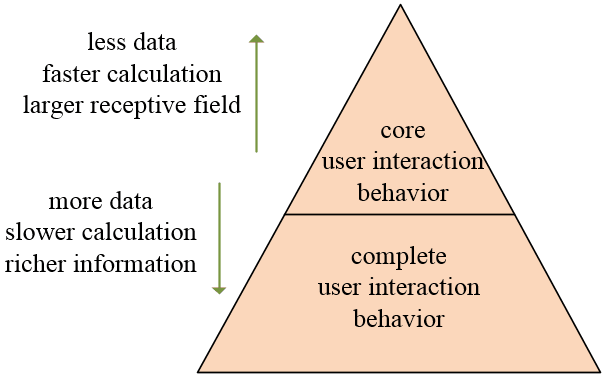
\includegraphics[width=7.2cm]{media/user-inter-behav-hierachy}
  \caption{User interaction behavior hierarchy.}
  \label{fig:user-inter-behav-hierachy}
\end{figure}

\begin{figure}[h]
  \centering
  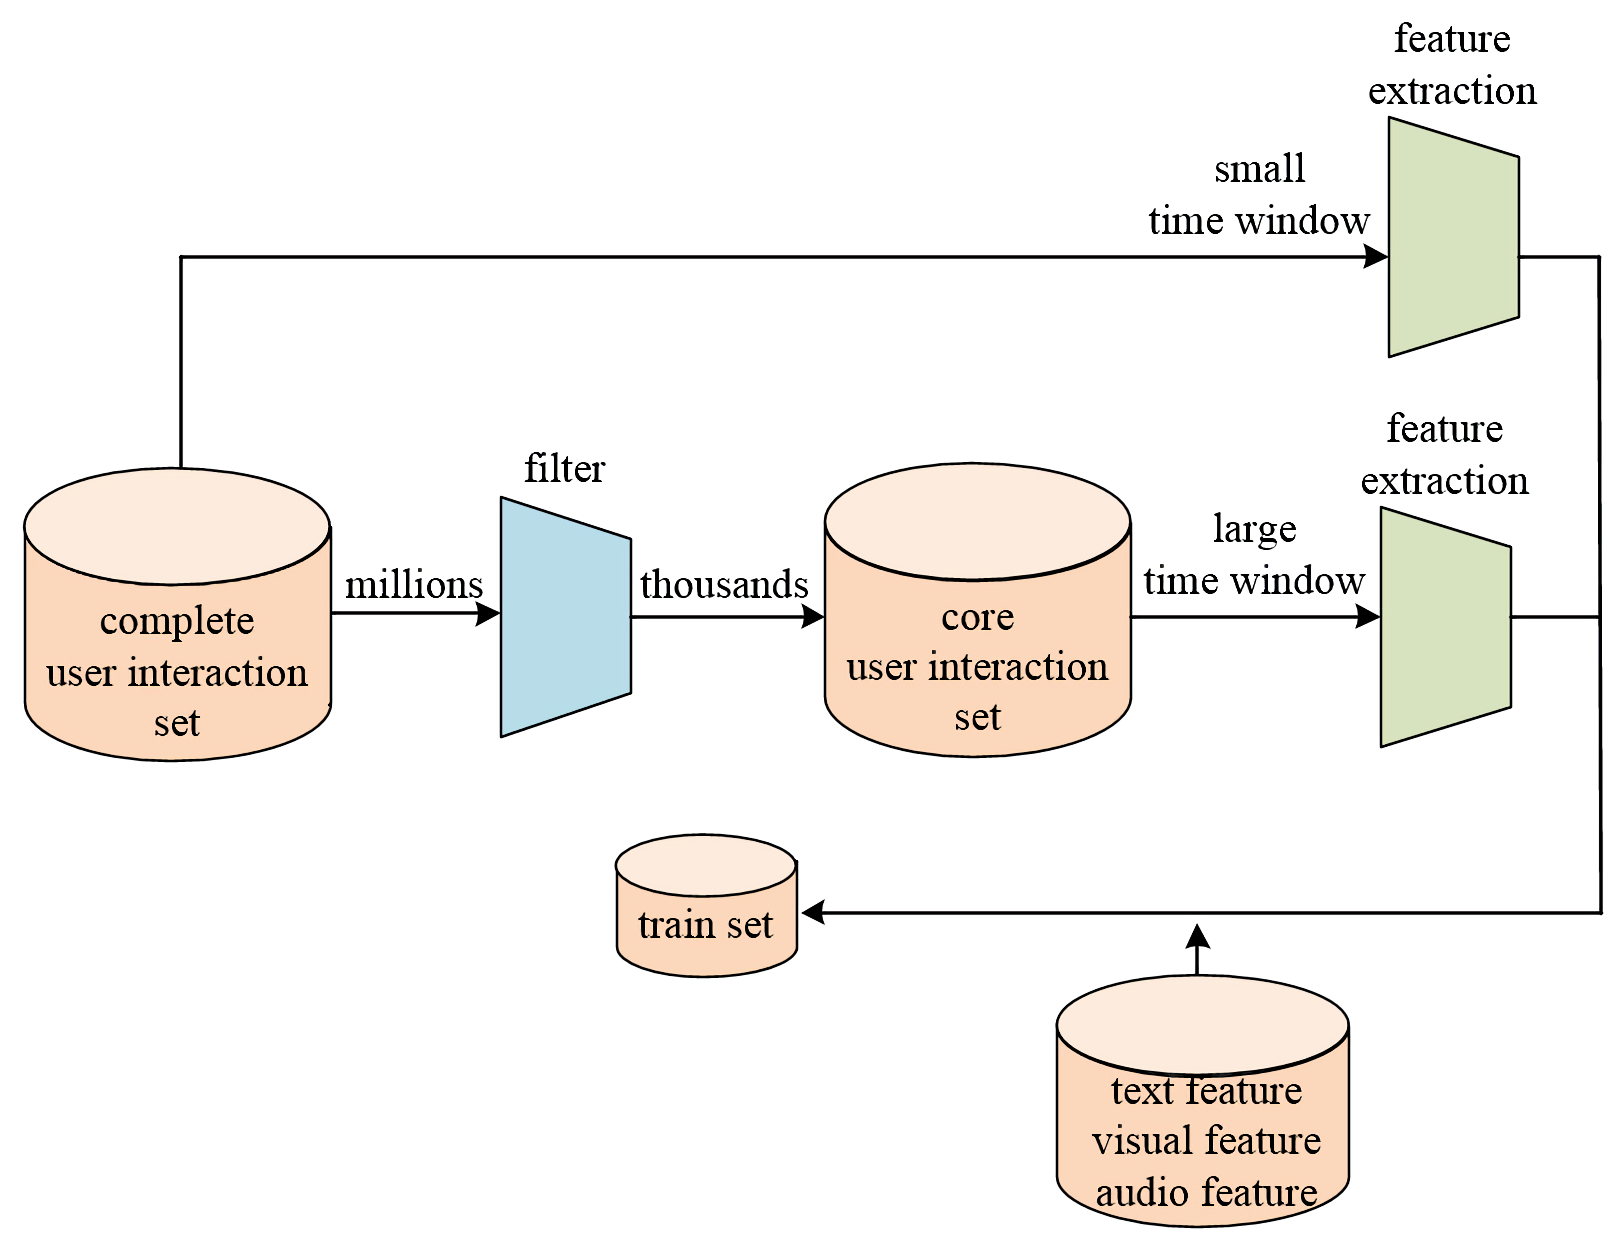
\includegraphics[width=8.5cm]{media/feat-extraction}
  \caption{Complete process of feature extraction.}
  \label{fig:feat-extraction}
\end{figure}


\subsection{Model Transfer}
\label{sec:model-transfer}

A basic assumption in time series prediction problem is the smoothness of the series, which means the values of neighboring time slots are close to each other. This assumption is also applicable to users' behaviors. Therefore, when selecting the training set and validation set, we will choose the data that are closer to the test set in time. For the training data that are distant from the test set, large difference might exist between the distribution of data, and it is crucial to make better use of them.

\begin{figure*}[h!]
  \centering
  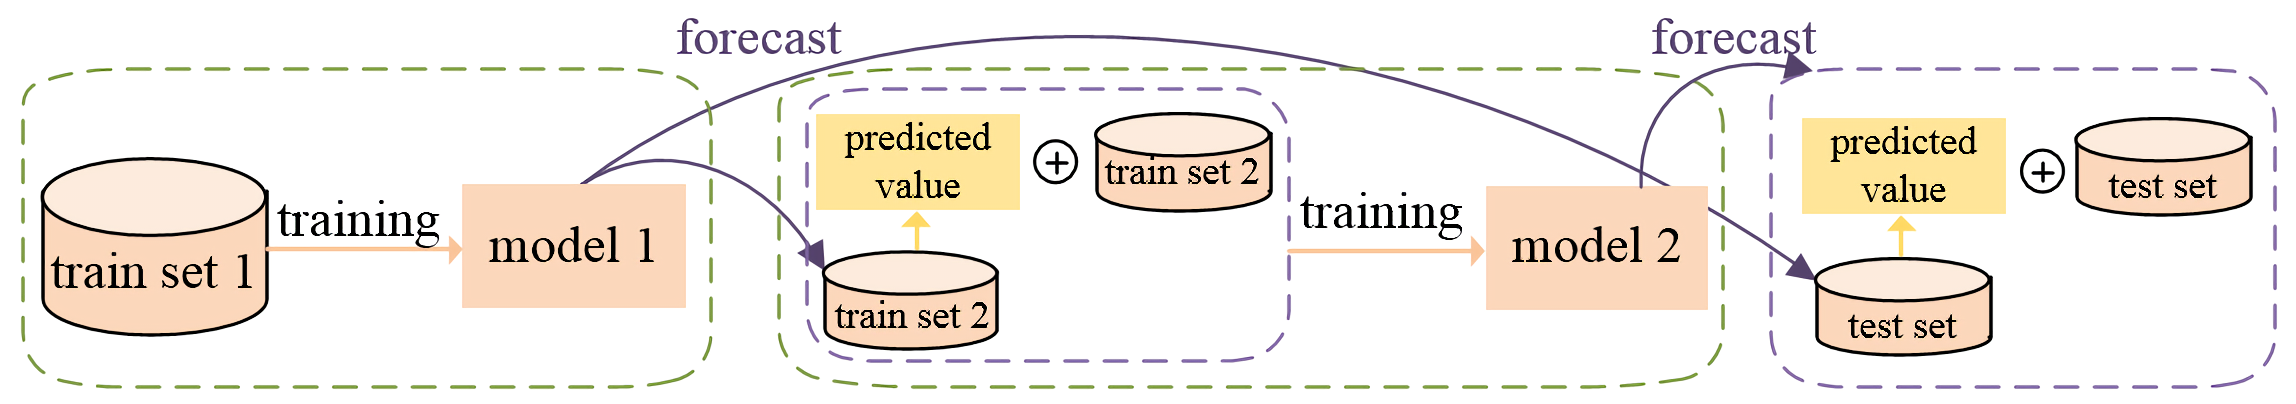
\includegraphics[width=17.3cm]{media/model-transfer}
  \caption{Procedures of the model transfer strategy.}
  \label{fig:model-transfer}
\end{figure*}

Suppose that there are two training sets, i.e., training set 1 and training set 2, and the latter of them is closer to the test set in time. Normally, the model trained on training set 2 will have a higher accuracy. Currently, there are two methods to deal with these two sets:

\begin{itemize}
  \item
    Directly combine training set 1 and 2. However, it is likely that the distributions of the data in the two sets are differently from each other. Thus, the data form training set 1 can bring plenty of noise, leading to a decrease in prediction results.
  \item
    Train models on training set 1 and 2 separately. The final results are often obtained through weighting the results of them. The defects of this method are two-fold. Firstly, weighting is unsuitable for evaluation metrics like AUC. Secondly, it can be hard to determine the weighting coefficients.
\end{itemize}

Hence, we proposed a model transfer strategy, to handle the disadvantages of traditional approaches. As illustrated in Fig.~\ref{fig:model-transfer}, this approach contains following steps:

\begin{itemize}
\item
  \emph{STEP 1}. Train Model 1 on training set 1.
\item
  \emph{STEP 2}. Predict training set 2 and test set using Model 1, and the prediction result is treated as a new feature.
\item
  \emph{STEP 3}. Train Model 2 on training set 2 based on both raw features and the new feature.
\item
  \emph{STEP 4}. Predict test set using Model 2, where the test set also contains both raw features and the new feature.
\end{itemize}

Instead of directly weighting the results of Model 1 and Model 2, we
treat the prediction result of Model 1 as an additional feature. Then,
using Model 2, the contribution of Model 1 to the final results can be
learned.


\subsection{Rank-Based Ensemble Approach}
\label{sec:rank-based-ensemble-approach}

In many machine learning works, the predictions are made solely depending on a single base model, but a superior accuracy will be reached if the results of multiple base models can be combined, even if each of them alone can only generate a moderate accuracy \cite{dietterich_ensemble_2000}. To achieve this goal, many ensemble models have been designed, the most famous of which include bagging \cite{breiman_bagging_1996}, boosting \cite{drucker_improving_1997}, and stacking \cite{wolpert_stacked_1992}.

For example, in stacking, several unique learners can be fused through a combiner, termed as a meta-learner. Given sample $x$, the stacking ensemble model can be formulated as Equation~\ref{eq:stacking}.
%
\begin{equation}
  F(x) = L\big(f_1(x), f_2(x), \ldots, f_n(x)\big)
  \label{eq:stacking}
\end{equation}
%
where $L(\cdot)$ denotes a second-level learner, $f_i$ denotes the $i$-th base model, and $K$ denotes the number of base models.

However, if the base models are ensembled through another learning model, the overall computational complexity can be high, while the accuracy improvement is modest. As a result, the preferred method in practical applications is Simple Averaging, which is a straightforward yet effective ensemble method. For sample $x$, the simple averaging ensemble model can be formulated as follows:
%
\begin{equation}
  F'(x) = \frac{1}{K} \sum_{i=1}^K {f_i(x)}
\end{equation}
%
where $f_i$ denotes the $i$-th base model, and $K$ denotes the number of base models.
In addition, none of the existing ensemble methods, including stacking and simple averaging, is capable of handling ensemble problems based on the AUC metric, which is equivalent to the probability that a randomly chosen positive example is ranked higher than a randomly chosen negative example. Therefore, we proposed a novel ensemble method based on rank to bridge this gap. For sample $x$, the rank-based ensemble model can be formulated as follows:
%
\begin{equation}
  F''(x) = \frac{1}{K} \sum_{i=1}^K \frac{\text{rank}\big( f_i(x) \big)}{\text{length}\big( f_i(x) \big)}
\end{equation}
%
where $f_i$ denotes the $i$-th base model, and $K$ denotes the number of base models. $\text{rank}(\cdot)$ represents the rank of the result among all the results, and $\text{length}(\cdot)$ represents the size of prediction results. The results of the rank-based ensemble method are listed in Table~\ref{table:res-rank-ensemble}.

\begin{table}[h!]
  \small
  \caption{Illustration of rank-based ensemble method.}
  \vspace{2pt}
  \label{table:res-rank-ensemble}
  \begin{center}
  \begin{tabular}{|c|c|c|c|c|c|}
  \hline
    ID & \begin{tabular}[c]{@{}c@{}} Like\\ probability$^\text{\emph{a}}$\end{tabular} & \begin{tabular}[c]{@{}c@{}} Like\\ probability$^\text{\emph{b}}$\end{tabular} & Rank$^\text{\emph{a}}$ & Rank$^\text{\emph{b}}$ & Final\\
    \hline
    1 & 0.044446 & 0.004366 & 2 & 2 & 0.4\\
    \hline
    2 & 0.331468 & 0.049055 & 4 & 3 & 0.7\\
    \hline
    3 & 0.042291 & 0.003703 & 1 & 1 & 0.2\\
    \hline
    4 & 0.129628 & 0.051494 & 3 & 4 & 0.7 \\
    \hline
    5 & 0.477071 & 0.135568 & 5 & 5 & 1.0\\
    \hline
  \end{tabular}
  \end{center}
\end{table}

It can be observed that, for sample 1, the prediction result of Model \emph{a} is approximately ten times as much as that of Model \emph{b}. Apparently, the simple averaging method is unreasonable for ensemble. In contrast, the proposed rank-based ensemble is capable of retaining the relative ranks of prediction results. For example, the predicted ranks of sample 1 are both 2 for the two models. Therefore, it is more suitable for tasks based on the evaluation metric of AUC.


%%%%%%%%%%%%%%%%%%%%%%%%%%%%%%%%%%%%%%%%%%%%%%%%%%%%%%%%%%%%%
%%%%%%%%%%%%%%%%%%%%%%%%%%%%%%%%%%%%%%%%%%%%%%%%%%%%%%%%%%%%%

\section{Experiment and Result}
\label{sec:experiment-and-result}

We evaluated our proposed method on the data of ICME Short Video Understanding Challenge (Track1). The dataset contains over 270 million user interaction behavior records in around nine days, 1.6\% of which correspond to the ‘like’ behaviors and 28\% of which finished watching the video. In the test set, approximately 39 million user-video pairs need to be predicted. For the user interaction data, we designed a number of statistical features from multiple perspectives, including the user, video, and author. For example, the total number of ‘like’ behaviors in the historical records of users. Regarding visual and audio features, PCA, Truncated SVD \cite{manning_matrix_2008}, and random projection \cite{dasgupta_experiments_2000} were utilized to reduce the dimensionality of the 128-dimensional raw feature vector. As to text features, the word frequency information was transformed into feature vectors using TFIDF and Word2vec. Finally, 30 million samples with 384-dimensional features were kept and used for the training of the model, the last 20\% of which were used for offline validation. Due to the considerable data size of Track 1 and our limited computational resource (with no GPU, small memory, and 2.4Ghz clock rate), we were only able to train a single LightGBM model \cite{ke_lightgbm:_2017}, which is less memory-demanding. Providing that better computational devices are available, deep learning models like DeepFM \cite{guo_deepfm:_2017} are also worth utilizing and improving. The performances of different models are listed in Table~\ref{table:perform-comparison} and Table~\ref{table:perform-comparison-ensemble}, where the AUCs are the real scores on the leaderboard of the competition.

It should be pointed out that, with only four days to go, the competition organizers made a significant revision to the competition rule, that is, from one submission per team per day to 10 submissions per team member per day. Moreover, the deadlines for the competition and team merge were both postponed. In other words, a team of five members can submit up to 50 submissions in a day. Before the revision of the rule, we ranked first with a large advantage over other teams, and our total submission number was 19 in one month, which was far less than others.

\begin{table}[h!]
  \small
  \caption{Performance comparison for different models.}
  \label{table:perform-comparison}
  \begin{center}
  \begin{tabular}{|c|l|c|c|}
  \hline
  Model & Descriptions & \begin{tabular}[c]{@{}l@{}}Task 1\\ (AUC)\end{tabular} & \begin{tabular}[c]{@{}l@{}}Task 2\\ (AUC)\end{tabular} \\ \hline
  IMWS  & \begin{tabular}[c]{@{}l@{}}Using \textbf{I}ncremental \textbf{M}ulti-\textbf{W}indow \\ \textbf{S}canning method. The baseline of \\ our proposed framework. We used \\ user behavior data from the prev-\\ ious two days.\end{tabular} & 0.7361 & 0.8748 \\
  \hline
  UIBH  & \begin{tabular}[c]{@{}l@{}}Added \textbf{U}ser \textbf{I}nteraction \textbf{B}ehavior \\ \textbf{H}ierarchy on the bias of baseline. \\ We used core behavior data from \\ the previous one week.\end{tabular} & 0.7537 & 0.8855 \\
  \hline
  MT & \begin{tabular}[c]{@{}l@{}}On the bias of the above model, \\ we added \textbf{M}odel \textbf{T}ransfer method.\end{tabular} & 0.7546 & 0.8860 \\
  \hline
  \end{tabular}
  \end{center}
\end{table}

\begin{table}[h!]
  \small
  \caption{Performance comparison for different ensemble methods.}
  \label{table:perform-comparison-ensemble}
  \begin{center}
  \begin{tabular}{|c|l|c|c|}
    \hline
    Model & Descriptions & \begin{tabular}[c]{@{}l@{}}Task 1\\ (AUC)\end{tabular} & \begin{tabular}[c]{@{}l@{}}Task 2\\ (AUC)\end{tabular} \\
    \hline
    Base model 1 & Base model 1 & 0.7399 & 0.8810 \\
    \hline
    Base model 2 & Base model 2 & 0.7427 & 0.8781 \\
    \hline
    Simple Averaging & \begin{tabular}[c]{@{}l@{}}Simple averaging\\ ensemble\end{tabular} & 0.7428 & 0.8801 \\
    \hline
  \end{tabular}
  \end{center}
\end{table}

%%%%%%%%%%%%%%%%%%%%%%%%%%%%%%%%%%%%%%%%%%%%%%%%%%%%%%%%%%%%%
%%%%%%%%%%%%%%%%%%%%%%%%%%%%%%%%%%%%%%%%%%%%%%%%%%%%%%%%%%%%%

\section{Conclusion}
\label{conclusion}

This paper investigated the short video recommendation problem in social media services. The main contributions of this research are the four techniques described in Section 3. The Incremental Multi-Window Scanning method enables us to extract user behavior features from different granularities and made our baseline method reach the top three in the leaderboard. However, the large time window during feature extraction may lead to substantial consumption of computing resources. Referring the memory hierarchy in computer architecture, the proposed User Interaction Behavior Hierarchy makes it possible to extract user behavior features with a larger time window based on core user interaction behavior. According to experimental results, not only is this method more than 50 times faster, but it significantly improves the prediction accuracy. Through Model Transfer, multiple base models can be combined to generate a better result. Our Rank-based Ensemble Method is significantly superior to the traditional simple averaging ensemble method in the task with the evaluation metric of AUC.

% References should be produced using the bibtex program from suitable
% BiBTeX files (here: strings, refs, manuals). The IEEEbib.bst bibliography
% style file from IEEE produces unsorted bibliography list.
% -------------------------------------------------------------------------
\bibliographystyle{IEEEbib}
\bibliography{ICME19-track1-rank3-submit}

\end{document}
